\documentclass[11pt]{amsart}

\usepackage[T1]{fontenc}
\usepackage{lmodern}
\usepackage{amssymb,amsmath}
\usepackage{booktabs,array}
\usepackage{graphicx}
\usepackage[dvipsnames]{xcolor}
\usepackage[margin=1.15in]{geometry}
\usepackage[colorlinks=true,linkcolor=blue!50!black,citecolor=blue!50!black,urlcolor=blue!50!black]{hyperref}

\newtheorem{theorem}{Theorem}[section]
\newtheorem{proposition}[theorem]{Proposition}
\newtheorem{lemma}[theorem]{Lemma}
\newtheorem{corollary}[theorem]{Corollary}
\theoremstyle{definition}
\newtheorem{definition}[theorem]{Definition}
\newtheorem{innerconj}{Conjecture}
\newenvironment{conjecture}[1]{\renewcommand{\theinnerconj}{#1}\innerconj}{\endinnerconj}
\theoremstyle{remark}
\newtheorem{remark}[theorem]{Remark}

\numberwithin{equation}{section}

\newcommand{\gt}{\gamma_t}
\newcommand{\ecc}{\operatorname{ecc}}
\newcommand{\iso}{\operatorname{iso}}
\newcommand{\comp}{\operatorname{c}}
\newcommand{\de}{\operatorname{de}}
\hypersetup{pdftitle={Counterexamples to five conjectures of Graffiti.pc on domination},pdfauthor={Deep Bhattacharjee}}
\providecommand{\doi}[1]{\url{https://doi.org/#1}}

\begin{document}

\title[Five conjectures of Graffiti.pc on domination]{Counterexamples to five conjectures\\ of Graffiti.pc on domination}

\author{Deep Bhattacharjee}
\address{Formerly, Electro-Gravitational Space Propulsion Laboratory (EGSPL),\newline Bhubaneswar, Odisha 751030, India}
\email{d.bhattacharjee@erl-forschung.de}
\email{itsdeep@live.com}
\urladdr{https://orcid.org/0000-0003-0466-750X}
\thanks{Corresponding author: \href{mailto:d.bhattacharjee@erl-forschung.de}{d.bhattacharjee@erl-forschung.de}; ORCID \href{https://orcid.org/0000-0003-0466-750X}{\mbox{0000-0003-0466-750X}}}

\subjclass[2020]{Primary 05C69; Secondary 05C05, 05C12}
\keywords{total domination, independent domination, well totally dominated graph, tree, caterpillar, Graffiti.pc, counterexample}

\begin{abstract}
Written on the Wall II, the list of conjectures of the program Graffiti.pc, records Conjectures 319, 352, 358, 359 and 427 as open. We show that all five are false. The counterexamples are caterpillars for Conjectures 352, 358, 359 and 427, and graphs built from complete graphs for Conjecture 319; each comes in an infinite family, and for Conjectures 358, 359 and 427 the difference between the two sides is unbounded.
\end{abstract}

\maketitle

\section{Introduction}

Graffiti.pc is a program written by DeLaVi\~na in 2001~\cite{DeLaVina2005a} after Fajtlowicz's Graffiti~\cite{Fajtlowicz1988}; it proposes inequalities between graph invariants that hold on its database of graphs. Its conjectures are collected, with their status, in DeLaVi\~na's list \emph{Written on the Wall~II}~\cite{WOWII}. Several hundred of them concern total domination, and some have been settled~\cite{DLPWW2007,DLPW2009,DesormeauxHenning2016}. This note disproves five conjectures that the list still marks as open (in its version of 26 July 2026): four on total domination and one on independent domination. The proofs are by hand. As in~\cite{BMB2026}, every finite statement is also re-checked by computer and in the Lean proof assistant; the computations are described in Section~\ref{sec:search} and Appendix~\ref{app:verification}.

All graphs are finite, simple and connected. For a vertex $v$ of $G$, $N(v)$ is its set of neighbours and $N[v]=N(v)\cup\{v\}$; for $X\subseteq V(G)$, $N(X)=\bigcup_{v\in X}N(v)$ and $\langle X\rangle$ is the subgraph induced by $X$. A set $D$ is \emph{dominating} if every vertex outside $D$ has a neighbour in $D$, and \emph{totally dominating} if every vertex of $G$ has a neighbour in $D$. The domination number $\gamma(G)$ and the total domination number $\gt(G)$ are the least sizes of such sets~\cite{CDH1980,HenningYeo2013}; the independent domination number $i(G)$ is the least size of a dominating set that is independent. A total dominating set is \emph{minimal} if no proper subset is a total dominating set; since every superset of a total dominating set is one, this holds as soon as no single vertex can be removed. $G$ is \emph{well totally dominated} if all its minimal total dominating sets have the same size~\cite{BEG2021}. A \emph{pendant} vertex or \emph{leaf} has degree one, and a \emph{support vertex} is a neighbour of a leaf. We write $d(u,v)$ for the distance, $\ecc(v)=\max_u d(v,u)$ for the eccentricity, and $C(G)$ for the \emph{center}, the set of vertices of least eccentricity. Following~\cite{WOWII}, the eccentricity of a set $X$ is
\[
\ecc(X)=\max_{v\notin X}\ \min_{x\in X} d(v,x).
\]
The number of vertices at even distance from $v$, including $v$ itself, is denoted $\de(v)$; the list calls it $\mathrm{dist}_{\mathrm{even}}(v)$. In a tree $T$, $L(T)$ is the set of leaves, $S(T)$ the set of support vertices, $D_2(T)$ the set of vertices of degree two, and $M(T)$ the set of vertices of maximum degree. Finally $\iso(H)$ and $\comp(H)$ are the numbers of isolated vertices and of components of a graph $H$.

The five conjectures read as follows in~\cite{WOWII}.

\begin{conjecture}{352}\label{c352}
If $T$ is a tree on $n>2$ vertices, then $\gt(T)\ge \comp\langle N(D_2)\cup D_2\rangle+\bigl\lceil\tfrac12\,\ecc_{\mathrm{avg}}(M)\bigr\rceil$, where $\ecc_{\mathrm{avg}}(M)$ is the average eccentricity of the vertices of maximum degree.
\end{conjecture}

\begin{conjecture}{358}\label{c358}
If $T$ is a tree on $n>2$ vertices, then $\gt(T)\ge\tfrac12\ecc(C)+\iso\langle S\rangle$.
\end{conjecture}

\begin{conjecture}{359}\label{c359}
If $T$ is a tree on $n>2$ vertices, then $\gt(T)\ge\tfrac12\ecc(C)+\comp\langle S\cup L\rangle$.
\end{conjecture}

\begin{conjecture}{319}\label{c319}
If $G$ has $n>1$ vertices and $\max_v\de(v)=\gamma(G)$, then $G$ is well totally dominated.
\end{conjecture}

\begin{conjecture}{427}\label{c427}
If $G$ has $n>3$ vertices, then $i(G)\le|E(C,V-C)|+\bigl\lfloor\tfrac23\,|E\langle V-N(P)\rangle|\bigr\rfloor$, where $P$ is the set of pendant vertices, $E\langle X\rangle$ is the edge set of $\langle X\rangle$ and $E(C,V-C)$ the set of edges with exactly one end in $C$.
\end{conjecture}

The printed statement of Conjecture~\ref{c427} introduces the set $M$ of maximum-degree vertices and then uses the symbols $C$ and $P$ without defining them. In the neighbouring entries of the list, $C$ is the center (Conjectures 430a--c) and $P$ the set of pendant vertices (Conjecture 425d); we read the statement this way, and we show in Theorem~\ref{thm:427} that it fails also if $C$ stands for $M$.

\begin{theorem}\label{thm:main}
Conjectures~\ref{c352}, \ref{c358}, \ref{c359}, \ref{c319} and~\ref{c427} are false. More precisely:
\begin{enumerate}
\item for $a\equiv 3$ and $r\equiv 0\pmod 4$ with $r\ge4$, the caterpillar $T(a,r)$ on $a+r+11$ vertices has $\gt=\frac{a+r+7}2$, one less than the right side of Conjecture~\ref{c352} (Theorem~\ref{thm:352});
\item for odd $k\ge3$, the caterpillar $Q_k$ on $7k-2$ vertices has $\gt=3k$, while the right sides of Conjectures~\ref{c358} and~\ref{c359} both equal $3k+\frac{k-1}4$ (Theorem~\ref{thm:358});
\item for $k\ge3$, the graph $G_k$ on $3k+1$ vertices satisfies $\de(v)=\gamma(G_k)=k+1$ for every vertex $v$, and has minimal total dominating sets of sizes $k+1$ and $2k$ (Theorem~\ref{thm:319});
\item for $m\ge2$, the caterpillar $H_m$ on $4m+1$ vertices has $i=2m$, while the right side of Conjecture~\ref{c427} equals $2$ (Theorem~\ref{thm:427}).
\end{enumerate}
\end{theorem}

The smallest counterexamples are $T(3,4)$ with $18$ vertices, $Q_3$ with $19$, $G_3$ with $10$, and an $8$-vertex tree for Conjecture~\ref{c427}. An exhaustive search (Section~\ref{sec:search}) shows that $T(3,4)$ and $Q_3$ are the only counterexamples of their orders and that there are none smaller. Likewise $G_3$ is the only counterexample to Conjecture~\ref{c319} with at most $11$ vertices, and the $8$-vertex tree the only counterexample to Conjecture~\ref{c427} with at most $8$ vertices.

\section{Two tools}

\begin{lemma}\label{lem:support}
Every total dominating set of a tree contains all its support vertices, and every dominating set meets $\{s\}\cup(N(s)\cap L)$ for each support vertex $s$.
\end{lemma}

\begin{proof}
A leaf $\ell$ has the single neighbour $s$, so a total dominating set must contain $s$, and a dominating set must contain $\ell$ or $s$.
\end{proof}

\begin{lemma}\label{lem:count}
Let $D$ be a total dominating set of a graph, $R$ a set of vertices, and $Q$ a set of vertices whose neighbours all lie in $R$. If every vertex of $R$ has at most two neighbours in $Q$, then $|D\cap R|\ge|Q|/2$.
\end{lemma}

\begin{proof}
Each $q\in Q$ has a neighbour in $D$, which lies in $D\cap R$. Counting the pairs $(q,x)$ with $q\in Q$, $x\in D\cap R$ and $qx$ an edge gives $|Q|\le\sum_{x\in D\cap R}|N(x)\cap Q|\le2|D\cap R|$.
\end{proof}

We also use Jordan's theorem~\cite{Jordan1869}: the center of a tree consists of the middle vertex, or the two middle vertices, of any longest path.

\section{Conjecture 352}\label{sec:352}

\begin{definition}
For $a,r\ge1$ let $T(a,r)$ be the tree formed by a path
\[
h,\ x_1,\dots,x_a,\ s_1,\ s_2,\ s_3,\ y_1,\dots,y_r,\ z
\]
together with three leaves attached to $h$ and one leaf $\ell_i$ attached to each $s_i$ (Figure~\ref{fig:t34}). It has $a+r+11$ vertices.
\end{definition}

\begin{figure}[t]
\centering
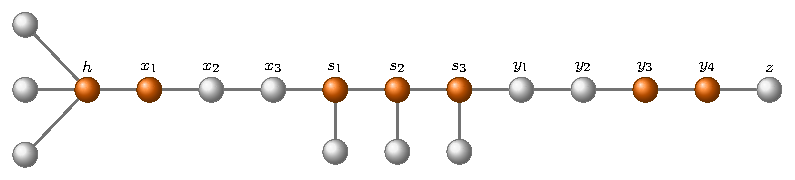
\includegraphics[width=0.92\textwidth]{figures/t34}
\caption{$T(3,4)$, the smallest counterexample to Conjecture~\ref{c352}. The shaded vertices form a total dominating set of size $7$; the right side of the conjecture is $8$.}
\label{fig:t34}
\end{figure}

\begin{theorem}\label{thm:352}
Let $a\equiv3\pmod 4$ and $r\equiv0\pmod 4$, $r\ge4$. Then
\[
\gt(T(a,r))=\frac{a+r+7}2<\frac{a+r+9}2=\comp\langle N(D_2)\cup D_2\rangle+\Bigl\lceil\frac12\ecc_{\mathrm{avg}}(M)\Bigr\rceil .
\]
\end{theorem}

\begin{proof}
Write $T=T(a,r)$. The vertex $h$ has degree $4$, the vertices $s_1,s_2,s_3$ have degree $3$, the $x_i$ and $y_j$ have degree $2$, and all other vertices are leaves. Hence $M=\{h\}$, and $\ecc(h)=d(h,z)=a+r+4$, since every other vertex is closer to $h$. As $a+r$ is odd, $\lceil\frac12\ecc(h)\rceil=\frac{a+r+5}2$. Next, $D_2=\{x_1,\dots,x_a,y_1,\dots,y_r\}$ and
\[
N(D_2)\cup D_2=\{h,x_1,\dots,x_a,s_1\}\cup\{s_3,y_1,\dots,y_r,z\}.
\]
The two sets on the right induce paths, and no edge joins them because $s_2$ lies in neither and $s_1s_3$ is not an edge. So $\comp\langle N(D_2)\cup D_2\rangle=2$, and the right side of Conjecture~\ref{c352} equals $\frac{a+r+9}2$.

\emph{Upper bound.} The set
\[
D=\{h,x_1,s_1,s_2,s_3\}\cup\{x_{4j},x_{4j+1}:1\le j\le\tfrac{a-3}4\}\cup\{y_{4j-1},y_{4j}:1\le j\le\tfrac r4\}
\]
has $5+\frac{a-3}2+\frac r2=\frac{a+r+7}2$ elements. It is a total dominating set: $h$ dominates its leaves and $x_1$; $x_1$ dominates $h$ and $x_2$; for $j\ge1$ the pair $x_{4j},x_{4j+1}$ dominates $x_{4j-1},\dots,x_{4j+2}$, so that $x_1,\dots,x_{a-1}$ are all dominated; $s_1$ dominates $x_a$, $\ell_1$ and $s_2$; $s_2$ dominates $s_1$, $s_3$ and $\ell_2$; $s_3$ dominates $s_2$, $\ell_3$ and $y_1$; and the pair $y_{4j-1},y_{4j}$ dominates $y_{4j-2},\dots,y_{4j+1}$, where $y_{r+1}$ means $z$.

\emph{Lower bound.} Let $D$ be any total dominating set. By Lemma~\ref{lem:support}, $h,s_1,s_2,s_3\in D$. Apply Lemma~\ref{lem:count} to $R_1=N(h)\cup\{x_2,\dots,x_a\}$ and $Q_1=\{h,x_2,\dots,x_{a-1}\}$: the neighbours of $h$ and of each $x_i$ with $2\le i\le a-1$ lie in $R_1$, and a vertex of $R_1$ is adjacent to at most two vertices of $Q_1$. Hence $|D\cap R_1|\ge\frac{a-1}2$. Likewise, with $R_2=\{y_1,\dots,y_r,z\}$ and $Q_2=\{y_2,\dots,y_r,z\}$, $|D\cap R_2|\ge\frac r2$. The sets $\{h,s_1,s_2,s_3\}$, $R_1$ and $R_2$ are disjoint, so $|D|\ge4+\frac{a-1}2+\frac r2=\frac{a+r+7}2$.
\end{proof}

\section{Conjectures 358 and 359}\label{sec:358}

\begin{definition}
For $k\ge1$ let $Q_k$ be the caterpillar whose spine is the path
\[
s_1,c_1,s_1',\ u_1,w_1,\ s_2,c_2,s_2',\ u_2,w_2,\ \dots,\ u_{k-1},w_{k-1},\ s_k,c_k,s_k'
\]
with one leaf attached to each $s_j$ and to each $s_j'$ (Figure~\ref{fig:q3}). It has $7k-2$ vertices. We call $\{s_j,c_j,s_j'\}$ the $j$-th block.
\end{definition}

\begin{figure}[t]
\centering
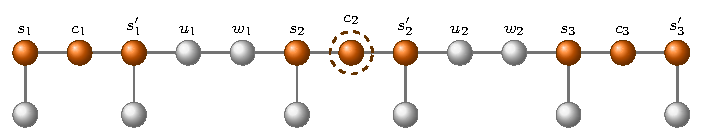
\includegraphics[width=0.92\textwidth]{figures/q3}
\caption{$Q_3$, the smallest counterexample to Conjectures~\ref{c358} and~\ref{c359}. The center $c_2$ is circled; the shaded vertices form a total dominating set of size $9$, while both conjectures demand $\frac{19}2$.}
\label{fig:q3}
\end{figure}

\begin{theorem}\label{thm:358}
Let $k\ge3$ be odd. Then $\gt(Q_k)=3k$, $\ecc(C)=\frac{5k-1}2$ and $\iso\langle S\rangle=\comp\langle S\cup L\rangle=2k$. Hence the right side of both Conjecture~\ref{c358} and Conjecture~\ref{c359} equals $3k+\frac{k-1}4>\gt(Q_k)$.
\end{theorem}

\begin{proof}
The leaves are the $2k$ attached vertices, so $S=\{s_j,s_j':1\le j\le k\}$. Two support vertices are at distance at least $2$ (they are separated by $c_j$ or by $u_j,w_j$), so $\langle S\rangle$ has no edges and $\iso\langle S\rangle=2k$; in $\langle S\cup L\rangle$ each support vertex is joined only to its own leaf, so $\comp\langle S\cup L\rangle=2k$.

The spine has $2k+3(k-1)=5k-3$ edges, and every vertex lies on the spine or is a leaf attached to it; the spine ends $s_1$ and $s_k'$ carry leaves. So the path from the leaf at $s_1$ to the leaf at $s_k'$, of length $5k-1$, is a longest path. Since $k$ is odd, $5k-1$ is even, and by Jordan's theorem $C$ is the single vertex at distance $\frac{5k-1}2$ from both ends; this is $c_m$ with $m=\frac{k+1}2$, because the leaf at $s_1$ is at distance $1+5(m-1)+1=\frac{5k-1}2$ from $c_m$. Thus $\ecc(C)=\ecc(c_m)=\frac{5k-1}2$.

The set $B$ of all $3k$ block vertices is a total dominating set: each leaf is dominated by its support vertex, $s_j$ and $s_j'$ by $c_j$, $c_j$ by $s_j$, $u_j$ by $s_j'$, and $w_j$ by $s_{j+1}$. Conversely, let $D$ be a total dominating set. By Lemma~\ref{lem:support}, $S\subseteq D$. For each $j$ the vertices $s_j,s_j'$ need neighbours in $D$, and these lie in $X_j=N(s_j)\cup N(s_j')$, which contains no support vertex. The sets $X_1,\dots,X_k$ are pairwise disjoint, because each vertex outside $S$ is adjacent to support vertices of only one block: $c_j$ to $s_j,s_j'$; $u_j$ to $s_j'$; $w_j$ to $s_{j+1}$; a leaf to its support vertex. Hence $|D|\ge2k+k=3k$, and $\gt(Q_k)=3k$.

Finally $\frac12\ecc(C)+2k=\frac{5k-1}4+2k=3k+\frac{k-1}4$.
\end{proof}

\begin{remark}
For even $k\ge4$ the center of $Q_k$ is the edge $u_{k/2}w_{k/2}$, $\ecc(C)=\frac{5k-2}2$, and the same argument gives right sides $3k+\frac{k-2}4>3k=\gt(Q_k)$. For $k=2$ the two sides are equal.
\end{remark}

\section{Conjecture 319}\label{sec:319}

\begin{definition}
For $k\ge3$ let $G_k$ consist of a complete graph on $c_1,\dots,c_k$, a vertex $x$, and for each $i$ a path $x,p_i,q_i,c_i$ (Figure~\ref{fig:g3}). It has $3k+1$ vertices.
\end{definition}

\begin{figure}[t]
\centering
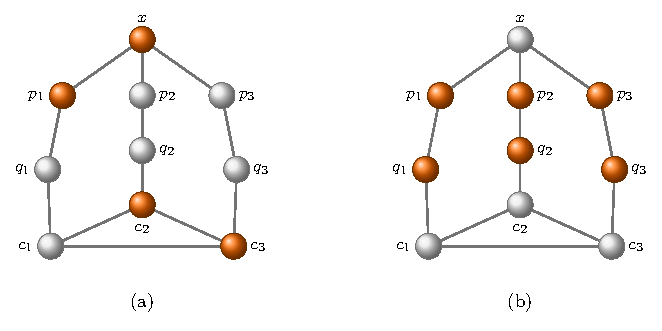
\includegraphics[width=0.78\textwidth]{figures/g3}
\caption{$G_3$, the smallest counterexample to Conjecture~\ref{c319}. Every vertex has four vertices at even distance (itself included) and $\gamma(G_3)=4$. The shaded sets are minimal total dominating sets of sizes $4$~(a) and $6$~(b).}
\label{fig:g3}
\end{figure}

\begin{theorem}\label{thm:319}
For $k\ge3$, every vertex $v$ of $G_k$ has $\de(v)=k+1$, and $\gamma(G_k)=\gt(G_k)=k+1$. The sets $\{x,p_1,c_2,\dots,c_k\}$ and $\{p_1,\dots,p_k,q_1,\dots,q_k\}$ are minimal total dominating sets of sizes $k+1$ and $2k$. Hence $G_k$ satisfies the hypothesis of Conjecture~\ref{c319} and is not well totally dominated.
\end{theorem}

\begin{proof}
\emph{Distances.} Let $i\neq j$. The following lists, read off from the paths through $x$ and through the clique, give the vertices at distance $1$, $2$ and $3$; no distance exceeds $3$.
\begin{center}
\begin{tabular}{lllll}
\toprule
vertex & distance $1$ & distance $2$ & distance $3$ & $\de$\\
\midrule
$x$ & $p_i$ & $q_i$ & $c_i$ & $1+k$\\
$p_i$ & $x,\ q_i$ & $p_j,\ c_i$ & $q_j,\ c_j$ & $1+(k-1)+1$\\
$q_i$ & $p_i,\ c_i$ & $x,\ c_j$ & $p_j,\ q_j$ & $1+1+(k-1)$\\
$c_i$ & $c_j,\ q_i$ & $p_i,\ q_j$ & $x,\ p_j$ & $1+1+(k-1)$\\
\bottomrule
\end{tabular}
\end{center}
For instance $d(p_i,c_j)=3$ along $p_i,q_i,c_i,c_j$, while the route through $x$ has length $4$; and $d(q_i,q_j)=3$ along $q_i,c_i,c_j,q_j$. In every row $\de=k+1$.

\emph{Domination.} The $k$ sets $N[q_i]=\{p_i,q_i,c_i\}$ are disjoint, so a dominating set $D$ has at least $k$ vertices. Suppose $|D|=k$. Then $D$ has exactly one vertex in each $N[q_i]$ and does not contain $x$, so $x$ is dominated by some $p_i\in D$. Then $c_i\notin D$ and $q_i\notin D$, so $c_i$ is dominated by some $c_j\in D$, $j\neq i$. But then $p_j,q_j\notin D$ and $x\notin D$, so $p_j$ is not dominated, a contradiction. Hence $\gamma(G_k)\ge k+1$.

The set $A=\{x,p_1,c_2,\dots,c_k\}$ is a total dominating set: $x$ is dominated by $p_1$; every $p_i$ by $x$; $q_1$ by $p_1$; $q_i$ by $c_i$ for $i\ge2$; $c_1$ by $c_2$; and $c_i$, $i\ge2$, by another $c_j$ with $j\ge2$, which exists since $k\ge3$. As $\gamma\le\gt\le|A|=k+1$, we get $\gamma(G_k)=\gt(G_k)=k+1$, and $A$ is minimal because it has the least possible size.

The set $B=\{p_1,\dots,p_k,q_1,\dots,q_k\}$ is a total dominating set: $x$ is dominated by $p_1$, $p_i$ and $q_i$ by each other, and $c_i$ by $q_i$. It is minimal: without $p_i$ the vertex $q_i$ has no neighbour in $B$, since $N(q_i)=\{p_i,c_i\}$; without $q_i$ the vertex $c_i$ has none, since $N(c_i)=\{q_i\}\cup\{c_j:j\neq i\}$. As $2k>k+1$, $G_k$ is not well totally dominated, while $\max_v\de(v)=k+1=\gamma(G_k)$.
\end{proof}

\begin{remark}
If $v$ itself is not counted in $\mathrm{dist}_{\mathrm{even}}(v)$, Conjecture~\ref{c319} already fails for the path $v_1v_2v_3v_4v_5$: the largest count is $2=\gamma(P_5)$, while $\{v_2,v_3,v_4\}$ and $\{v_1,v_2,v_4,v_5\}$ are minimal total dominating sets. So the conjecture is false under either reading; the definition in~\cite{WOWII} counts all vertices at even distance, which includes $v$.
\end{remark}

\section{Conjecture 427}\label{sec:427}

\begin{definition}
For $m\ge2$ let $H_m$ be the path $v_{-m},\dots,v_0,\dots,v_m$ with one leaf $\ell_j$ attached to each $v_j$, $j\neq0$; it has $4m+1$ vertices. For $m\ge3$ let $F_m$ be the path $v_1,\dots,v_m$ with one leaf attached to each $v_j$ and a second leaf attached to $v_2$; it has $2m+1$ vertices.
\end{definition}

\begin{figure}[t]
\centering
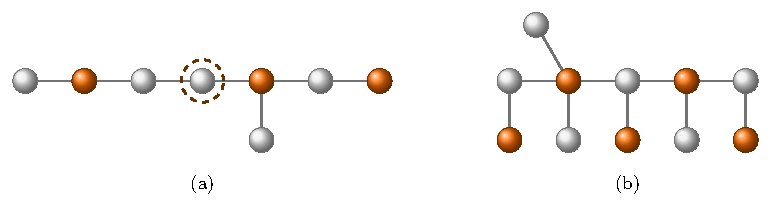
\includegraphics[width=0.92\textwidth]{figures/t8f5}
\caption{(a) The smallest counterexample to Conjecture~\ref{c427}: the right side is $2$ (the center is circled) and $i=3$, attained by the shaded set. (b) $F_5$: with $C$ read as the set of maximum-degree vertices the right side is $4$, while $i=5$.}
\label{fig:t8f5}
\end{figure}

\begin{theorem}\label{thm:427}
For $m\ge2$, the right side of Conjecture~\ref{c427} for $H_m$ equals $2$, while $i(H_m)=2m$. If $C$ is replaced by the set $M$ of maximum-degree vertices, the right side for $F_m$ equals $4$, while $i(F_m)=m$; so for $m\ge5$ the conjecture fails in this reading too.
\end{theorem}

\begin{proof}
In $H_m$ the path $\ell_{-m},v_{-m},\dots,v_m,\ell_m$ is a longest path, so $C=\{v_0\}$ by Jordan's theorem. As $v_0$ has degree $2$, $|E(C,V-C)|=2$. The pendant vertices are the $\ell_j$, so $N(P)=\{v_j:j\neq0\}$ and $V-N(P)=\{v_0\}\cup\{\ell_j\}$, an independent set; the second term vanishes and the right side is $2$. By Lemma~\ref{lem:support} an independent dominating set meets each of the $2m$ disjoint sets $\{v_j,\ell_j\}$, $j\neq0$, so $i(H_m)\ge2m$; and $\{v_j:j\text{ odd}\}\cup\{\ell_j:j\neq0\text{ even}\}$ is an independent dominating set of size $2m$ (it dominates $v_0$ through $v_{\pm1}$).

In $F_m$ the vertex $v_2$ has degree $4$ and every other vertex has degree at most $3$, so $M=\{v_2\}$ and $|E(M,V-M)|=4$. Every spine vertex is a support vertex, so $V-N(P)$ is the set of leaves, which is independent; the right side is $4$. By Lemma~\ref{lem:support}, $i(F_m)\ge m$, and the vertices $v_j$ with $j$ even together with the leaves at the $v_j$ with $j$ odd form an independent dominating set of size $m$.
\end{proof}

The smallest counterexample has $8$ vertices: the path $a_1a_2\cdots a_7$ with a leaf $b$ attached to $a_5$ (Figure~\ref{fig:t8f5}(a)). The path $a_1\cdots a_7$ is a longest path, so the center is $\{a_4\}$, which has degree $2$. The pendant vertices are $a_1$, $a_7$ and $b$, so $N(P)=\{a_2,a_5,a_6\}$, and $\langle V-N(P)\rangle$ has the single edge $a_3a_4$. The right side is $2+\lfloor\frac23\rfloor=2$. On the other hand $N[a_5]$ has four vertices and every other closed neighbourhood at most three, so two vertices dominate at most seven of the eight vertices; and $\{a_2,a_5,a_7\}$ is an independent dominating set. So $i=3$.

\section{Exhaustive search}\label{sec:search}

The trees with at most $24$ vertices ($63{,}242{,}254$ trees with $3$ to $24$ vertices) were generated with \texttt{gentreeg} from nauty~\cite{McKayPiperno2014}, which implements the algorithm of Wright, Richmond, Odlyzko and McKay~\cite{WROM1986}, and tested against Conjectures~\ref{c352}, \ref{c358} and~\ref{c359}; $\gt$ was computed by a dynamic programme over a rooted tree, and compared with a brute-force computation for all trees with at most $16$ vertices. Table~\ref{tab:search} gives the numbers of counterexamples. The connected graphs were generated with \texttt{geng}. Among the $1{,}018{,}690{,}328$ connected graphs with $2$ to $11$ vertices, $46$ satisfy the hypothesis of Conjecture~\ref{c319}, and $G_3$ is the only one of them that is not well totally dominated. Among the $11{,}989{,}760$ connected graphs with $4$ to $10$ vertices, Conjecture~\ref{c427} has $1$, $12$ and $72$ counterexamples with $8$, $9$ and $10$ vertices and none smaller; with $C$ read as $M$ it has $5$, all with $10$ vertices.

\begin{table}[t]
\centering
\caption{Counterexamples among all trees with $n$ vertices.}
\label{tab:search}
\begin{tabular}{rrrr}
\toprule
$n$ & trees & Conjecture~\ref{c352} & Conjectures~\ref{c358}, \ref{c359}\\
\midrule
$3$--$17$ & $81{,}135$ & $0$ & $0$\\
$18$ & $123{,}867$ & $1$ & $0$\\
$19$ & $317{,}955$ & $4$ & $1$\\
$20$ & $823{,}065$ & $13$ & $3$\\
$21$ & $2{,}144{,}505$ & $31$ & $14$\\
$22$ & $5{,}623{,}756$ & $73$ & $38$\\
$23$ & $14{,}828{,}074$ & $157$ & $108$\\
$24$ & $39{,}299{,}897$ & $318$ & $255$\\
\bottomrule
\end{tabular}
\end{table}

\appendix

\section{Verification}\label{app:verification}

The proofs above use no computation. The computer checks the finite claims about the smallest members of each family and the searches of Section~\ref{sec:search}, independently in four languages; all files are in the repository listed under Data and code availability.
\begin{enumerate}
\item \textbf{C.} Exhaustive searches: \texttt{search352.c} and \texttt{search358.c} over trees in graph6 format (total domination number by dynamic programming, optionally compared with brute force over all vertex subsets), \texttt{c319.c} and \texttt{c427.c} over connected graphs (all parameters by exhaustion over vertex subsets, in integer arithmetic). The search for Conjecture~\ref{c319} on the $1{,}006{,}700{,}565$ connected graphs with $11$ vertices was split into three parts with \texttt{geng}'s \texttt{res/mod} option.
\item \textbf{Python} (exact integer and rational arithmetic): for $T(a,r)$ with $a\in\{3,7,11\}$, $r\in\{4,8,12,16\}$, for $Q_k$ with odd $k\le11$, for $G_k$ with $k\le5$, for $H_m$ with $m\le5$ and for $F_m$ with $5\le m\le8$, recomputes every quantity in Theorems~\ref{thm:352}--\ref{thm:427} from the edge lists, and checks the stated values of $\gt$, $\gamma$ and $i$ by exhaustion for the smaller members.
\item \textbf{Julia}: the same quantities, with $\gt$, $\gamma$, $i$ and the minimal total dominating sets found by brute force over all vertex subsets (up to $2^{26}$ subsets), except that $\gt(Q_k)$ for $k\ge5$ is computed by a tree dynamic programme.
\item \textbf{Lean~4}: self-contained files without Mathlib. For $T(3,4)$, $Q_3$, $G_3$, the $8$-vertex tree and $F_5$ they compute the right sides of the conjectures from the edge lists and prove that the conjectures fail. The refutations of Conjectures~\ref{c352}, \ref{c358} and~\ref{c359} exhibit a total dominating set that is too small and depend on no axioms; those of Conjectures~\ref{c319} and~\ref{c427} evaluate $\gamma$ and $i$ over all vertex subsets in the kernel and depend only on \texttt{propext}. The exact values $\gt(T(3,4))=7$ and $\gt(Q_3)=9$ are also checked, by compiled evaluation (\texttt{native\_decide}); the refutations do not use them.
\end{enumerate}

\section*{Statements and Declarations}

\subsection*{Funding} No funding was received for conducting this study.

\subsection*{Competing interests} The author has no competing interests to declare that are relevant to the content of this article.

\subsection*{Data and code availability} The programs, their outputs and the Lean files are available at \url{https://github.com/creelie/eCY} and archived on Zenodo, \doi{10.5281/zenodo.23252219}.

\subsection*{Use of generative AI} The author used Claude (Anthropic) for programming, computation and drafting; the author checked the mathematics and takes full responsibility for the content.

{\raggedright
\begin{thebibliography}{99}

\bibitem{BEG2021}
S.~Bahad\i r, T.~Ekim and D.~G\"oz\"upek, \emph{Well-totally-dominated graphs}, Ars Math. Contemp. \textbf{20} (2021), 209--222. \doi{10.26493/1855-3974.2465.571}

\bibitem{BMB2026}
D.~Bhattacharjee, P.~Mandal and U.~Bhattacharya, \emph{Resolving Erd\H{o}s--Ulam monochromatic union-closed family conjectures}, preprint, 2026. \href{https://arxiv.org/abs/2610.02833}{arXiv:2610.02833}

\bibitem{CDH1980}
E.~J. Cockayne, R.~M. Dawes and S.~T. Hedetniemi, \emph{Total domination in graphs}, Networks \textbf{10} (1980), 211--219. \doi{10.1002/net.3230100304}

\bibitem{DeLaVina2005a}
E.~DeLaVi\~na, \emph{Graffiti.pc: a variant of Graffiti}, in: Graphs and Discovery, DIMACS Ser. Discrete Math. Theoret. Comput. Sci. 69, Amer. Math. Soc., Providence, RI, 2005, 71--79. \doi{10.1090/dimacs/069/05}

\bibitem{WOWII}
E.~DeLaVi\~na, \emph{Written on the Wall II (conjectures of Graffiti.pc)}, \url{http://cms.uhd.edu/faculty/delavinae/research/wowII/}; version of 26 July 2026 archived at \url{https://web.archive.org/web/20260726061534/http://cms.uhd.edu/faculty/delavinae/research/wowII/all.html}

\bibitem{DLPW2009}
E.~DeLaVi\~na, C.~E. Larson, R.~Pepper and B.~Waller, \emph{Graffiti.pc on the total domination number of a tree}, Congr. Numer. \textbf{195} (2009), 5--18.

\bibitem{DLPWW2007}
E.~DeLaVi\~na, Q.~Liu, R.~Pepper, B.~Waller and D.~B. West, \emph{Some conjectures of Graffiti.pc on total domination}, Congr. Numer. \textbf{185} (2007), 81--95.

\bibitem{DesormeauxHenning2016}
W.~J. Desormeaux and M.~A. Henning, \emph{Lower bounds on the total domination number of a graph}, J. Comb. Optim. \textbf{31} (2016), 52--66. \doi{10.1007/s10878-014-9708-2}

\bibitem{Fajtlowicz1988}
S.~Fajtlowicz, \emph{On conjectures of Graffiti}, Discrete Math. \textbf{72} (1988), 113--118. \doi{10.1016/0012-365X(88)90199-9}

\bibitem{HenningYeo2013}
M.~A. Henning and A.~Yeo, \emph{Total Domination in Graphs}, Springer Monographs in Mathematics, Springer, New York, 2013. \doi{10.1007/978-1-4614-6525-6}

\bibitem{Jordan1869}
C.~Jordan, \emph{Sur les assemblages de lignes}, J. Reine Angew. Math. \textbf{70} (1869), 185--190. \doi{10.1515/crll.1869.70.185}

\bibitem{McKayPiperno2014}
B.~D. McKay and A.~Piperno, \emph{Practical graph isomorphism, II}, J. Symbolic Comput. \textbf{60} (2014), 94--112. \doi{10.1016/j.jsc.2013.09.003}

\bibitem{WROM1986}
R.~A. Wright, B.~Richmond, A.~Odlyzko and B.~D. McKay, \emph{Constant time generation of free trees}, SIAM J. Comput. \textbf{15} (1986), 540--548. \doi{10.1137/0215039}

\end{thebibliography}
}

\end{document}
